\addbibresource{reference.bib}

\chapter{Testování}\label{chap:test}
V této kapitol bude čtenář seznámen s metodami testování pro zajištění kvality jednotlivých softwarových komponent a s provedenými experimenty.

%********************************************************************************
% Metody testování
%********************************************************************************
\section{Metody testování}
\subsection{Jednotkové testy}
Pro části jednotlivých softwarových komponent byly použity jednotkové testy \cite{testing_evans} (tzv. \textit{Unit testy}). Jednotkové testy jsou základním typem testu, který ověřuje funkčnost samostatně testovatelných částí systému - tzv. jednotek. Výhodou těchto testů je jejich automatizovatelnost. Byl použit \textit{JUnit} framework - framework pro jednotkové testy pro platformu Java. 

\subsection{Integrační testy}
Integrační testy byly použity pro ověření správné komunikace jednotlivých komponent systému, zejména pak handlera (viz \ref{chap:handler}) a backendové aplikace mastera (viz \ref{chap:master:backend}).

\subsection{Systémové testy}

%********************************************************************************
% Experimenty
%********************************************************************************
\section{Experimenty}
Pro ověření funkčnosti a dostatečné propustnosti systému bylo provedeno několik experimentů, které budou v této podkapitole popsány. Pro tyto experimenty byla použita dvě různá prostředí:
\begin{description}
    \item[localhost] -- jeden počítač, na kterém byl spuštěn emulátor, handler a master současně. Použití počítač má CPU 3 GHz Intel Core i7, 16 GB 1600 MHz DDR3 RAM a SSD disk o kapacitě \unit{500}{GB} (MacBook Pro).
    \item[CERN openstack] -- cloudová infrastruktura v CERN, kterou CERN poskytuje partnerským univerzitám a dalším institucím. Tato infrastruktura je založená na \textit{OpenStack} \textit{IaaS}\footnote{Z angl. \textit{Infrastructure as a Service}.} platformě, která umožňuje řízení výpočetního výkonu, úložiště a síťových prostředcích v datacentrech skrze webovou aplikaci nebo \textit{OpenStack API}.

    Byl vytvořen cluster s těmito virtuálními počítači:
    \begin{itemize}
        \item \texttt{pixnet-master.cern.ch} -- na tomto uzlu byla nasazena backendová aplikace mastera společně s webovým serverem, poskytujícím webový frontend mastera. Instance má 2~VCPU, \unit{4}{GB}~RAM a \unit{20}{GB} diskové kapacity.
        \item \texttt{pixnet-handler-1.cern.ch} -- uzel pro nasazení backendové aplikace handlera. Instance má 4~VCPU, \unit{8}{GB}~RAM a \unit{40}{GB} diskové kapacity.
        \item \texttt{pixnet-emulator-katherine1.cern.ch} -- uzel pro nasazení emulátoru vyčítacího rozhraní \textit{Katherine}. Instance má 1~VCPU, \unit{2}{GB}~RAM a \unit{10}{GB} diskové kapacity.
        \item \texttt{pixnet-emulator-katherine2.cern.ch} -- uzel pro nasazení emulátoru vyčítacího rozhraní \textit{Katherine}. Instance má 1~VCPU, \unit{2}{GB}~RAM a \unit{10}{GB} diskové kapacity.
    \end{itemize}

\end{description}

\subsection{Experiment první: zpracovávání fronty naměřených dat}


\begin{figure}[h]
    \centering
    \begin{subfigure}[t!]{0.47\textwidth}
        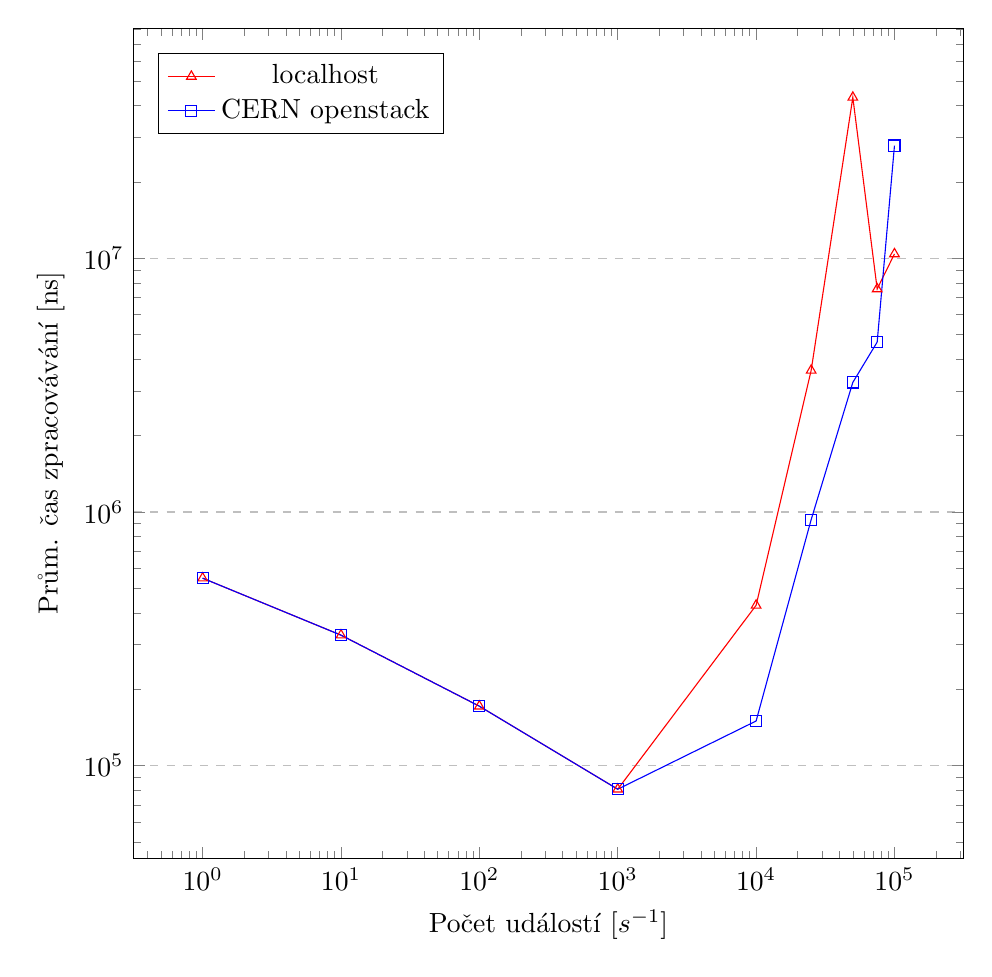
\begin{tikzpicture}
            \begin{loglogaxis}[
                xlabel={Počet událostí [$s^{-1}$]},
                ylabel={Prům. čas zpracovávání [ns]},
                legend pos=north west,
                ymajorgrids=true,
                grid style=dashed,
                width=\textwidth,
                height=\textwidth,
            ]
            \addplot[
                color=red,
                mark=triangle,
                ]
                coordinates {
                    (1,548539.5)
                    (10,327037.6097)
                    (100,171609.3892)
                    (1000,80747.81636)
                    (10000,428631.4967)
                    (25000,3616756.103)
                    (50000,43089381.58)
                    (75000,7572697.545)
                    (100000,10406080.54)
                };
            \addplot[
                color=blue,
                mark=square,
                ]
                coordinates {
                    (1,548539.5)
                    (10,327037.6097)
                    (100,171609.3892)
                    (1000,80747.81636)
                    (10000,150000.808)
                    (25000,933122.5602)
                    (50000,3242140.3333)
                    (75000,4674643.645)
                    (100000,27828674.3)
                };
            \legend{localhost,CERN openstack} 
            \end{loglogaxis}
        \end{tikzpicture}
        \caption{Závislost průměrné doby zpracování události na počtu událostí za sekundu.}
        \label{fig:test:arch}
    \end{subfigure}
    \hspace{0.2cm}
    \begin{subfigure}[t!]{0.47\textwidth}
    
        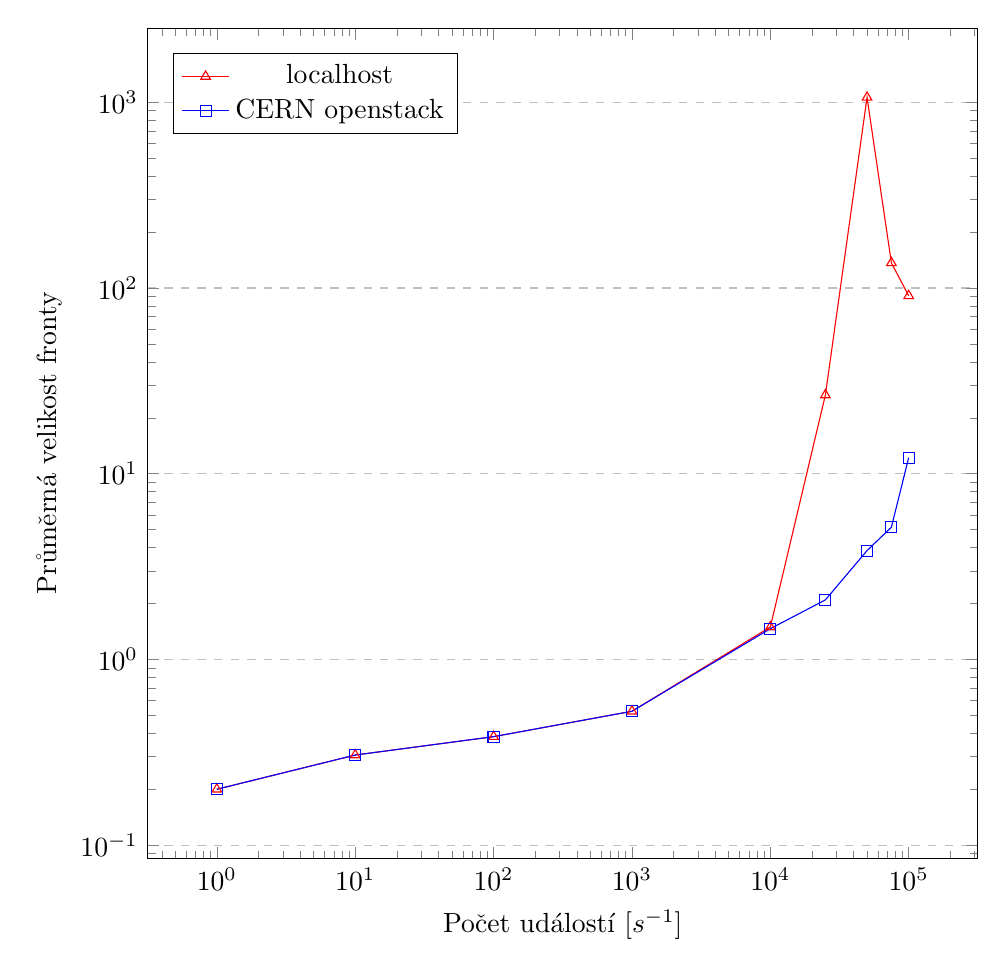
\begin{tikzpicture}
            \begin{loglogaxis}[
                xlabel={Počet událostí [$s^{-1}$]},
                ylabel={Průměrná velikost fronty},
                legend pos=north west,
                ymajorgrids=true,
                grid style=dashed,
                width=\textwidth,
                height=\textwidth,
            ]
            \addplot[
                color=red,
                mark=triangle,
                ]
                coordinates {
                    (1,0.2)
                    (10,0.305699482)
                    (100,0.383944154)
                    (1000,0.525876461)
                    (10000,1.495)
                    (25000,26.53898305)
                    (50000,1061.88027)
                    (75000,136.5602007)
                    (100000,90.73529412)
                };
            \addplot[
                color=blue,
                mark=square,
                ]
                coordinates {
                    (1,0.2)
                    (10,0.305699482)
                    (100,0.383944154)
                    (1000,0.525876461)
                    (10000,1.464106845)
                    (25000,2.091973244)
                    (50000,3.854271357)
                    (75000,5.154103853)
                    (100000,12.20805369)
                };
            \legend{localhost,CERN openstack}
            \end{loglogaxis}
        \end{tikzpicture}
        \caption{Závislost průměrné velikosti fronty s událostmi na počtu událostí za sekundu.}
        \label{fig:test:arch}
        
    \end{subfigure}
        
    \caption{Závislost průměrné doby zpracování událostí a jejich průměrnému počtu ve frontě na počtu událostí za sekundu.}
    \label{fig:test:arch}
\end{figure}

\begin{figure}[h]
    \centering
    \begin{tikzpicture}
        \begin{axis}[
          xmin = 0, xmax = 62000,
          ymin = 0,
          axis y line*=left,
          xlabel={Čas [ms]},
          xlabel near ticks,
          ylabel={Doba zpracování událostí [ns]},
          ylabel near ticks,
          width=0.90\textwidth,
          height=0.88\textwidth,
        ]
          \addplot[color=orange] table {figures/data/test_queue_waiting.dat};
          \label{plot_1_y1}
        \end{axis}
        \begin{axis}[
          xmin = 0, xmax = 62000,
          ymin = 0,% ymax = 11000,
          hide x axis,
          axis y line*=right,
          ylabel={Počet událostí ve frontě},
          ylabel near ticks,
          width=0.90\textwidth,
          height=0.88\textwidth,
        ]
        \addplot[color=gray] table {figures/data/test_queue_size.dat};
        \label{plot_1_y2}
        \addlegendimage{/pgfplots/refstyle=plot_1_y1}\addlegendentry{Doba zpracování událostí}
        \addlegendimage{/pgfplots/refstyle=plot_1_y2}\addlegendentry{Počet událostí ve frontě}
        \end{axis}
      \end{tikzpicture}

    \caption{Vývoj doby zpracovávání událostí a počtu událostí ve frontě v rámci \unit{60}{s} dlouhé akvizice, při konstantním generovaném množství událostí ($50000~s^{-1}$).}
    \label{fig:test:arch}
\end{figure}